
\documentclass{beamer}
\usecolortheme{dove}
\setbeamertemplate{navigation symbols}{}
\usepackage{amsmath,amssymb,amsfonts,amsthm, multicol, subfigure, color}
\usepackage{bm}
\usepackage{graphicx}
\usepackage{tabularx}
\usepackage{booktabs}
\usepackage{hyperref}
\usepackage{pdfpages}
\usepackage{xcolor}
\definecolor{seagreen}{RGB}{46, 139, 87}
\def\independenT#1#2{\mathrel{\rlap{$#1#2$}\mkern2mu{#1#2}}}
\newcommand\indep{\protect\mathpalette{\protect\independenT}{\perp}}
\def\log{\text{log}}
\newcommand\logit{\text{logit}}
\newcommand\iid{\stackrel{\text{iid}}{\sim}}
\newcommand\E{\text{E}}
\newcommand\V{\text{V}}
\renewcommand\P{\text{P}}
\newcommand{\Cov}{\text{Cov}}
\newcommand{\Cor}{\text{Cor}}
\newcommand\doop{\texttt{do}}
\usepackage{stackrel}
\usepackage{tikz}
\usetikzlibrary{arrows,shapes.arrows,positioning,shapes,patterns,calc}
\newcommand\slideref[1]{\vskip .1cm \tiny \textcolor{gray}{{#1}}}
\newcommand\red[1]{\color{red}#1}
\newcommand\blue[1]{\color{blue}#1}
\newcommand\gray[1]{\color{gray}#1}
\newcommand\seagreen[1]{\color{seagreen}#1}
\newcommand\purple[1]{\color{purple}#1}
\newcommand\orange[1]{\color{orange}#1}
\newcommand\black[1]{\color{black}#1}
\newcommand\white[1]{\color{white}#1}
\newcommand\teal[1]{\color{teal}#1}
\newcommand\magenta[1]{\color{magenta}#1}
\newcommand\Fuchsia[1]{\color{Fuchsia}#1}
\newcommand\BlueGreen[1]{\color{BlueGreen}#1}
\newcommand\bblue[1]{\textcolor{blue}{\textbf{#1}}}
\newcommand\bred[1]{\textcolor{red}{\textbf{#1}}}
\newcommand\bgray[1]{\textcolor{gray}{\textbf{#1}}}
\newcommand\bgreen[1]{\textcolor{seagreen}{\textbf{#1}}}
\newcommand\bref[2]{\href{#1}{\color{blue}{#2}}}
\colorlet{lightgray}{gray!40}
\pgfdeclarelayer{bg}    % declare background layer for tikz
\pgfsetlayers{bg,main} % order layers for tikz
\newcommand\mycite[1]{\begin{scriptsize}\textcolor{darkgray}{(#1)}\end{scriptsize}}
\newcommand{\tcframe}{\frame{
%\small{
\only<1|handout:0>{\tableofcontents}
\only<2|handout:1>{\tableofcontents[currentsubsection]}}
%}
}

\newcommand{\goalsframe}{\begin{frame}{Learning goals for today}
By the end of class, you will be able to
\begin{itemize}
    \item explain key ideas of data collection
    \begin{itemize}
    \item target population
    \item sampling frame
    \item undercoverage
    \item simple random sample
    \item unequal probability sample
    \end{itemize}
\end{itemize} \vskip .2in
\end{frame}}

\usepackage[round]{natbib}
\bibliographystyle{humannat-mod}
\setbeamertemplate{enumerate items}[default]
\usepackage{mathtools}

\title{Studying Social Inequality with Data Science}
\author{Ian Lundberg}
\date{\today}

\begin{document}

\begin{frame}
\begin{tikzpicture}[x = \textwidth, y = \textheight]
\node at (0,0) {};
\node at (1,1) {};
\node[anchor = north west, align = left, font = \huge] at (0,.9) {Social Data Science};
\node[anchor = north east, align = right] (number) at (1,.9) {SOCIOL 114\\Winter 2025};
\node[anchor = north, font = \Large, align = right] at (.5,.5) {\bblue{Sampling for Population Inference}};
\end{tikzpicture}
\end{frame}

\begin{frame}
When you think of data science,\\
what kind of data do you think of?
\end{frame}

\goalsframe

\begin{frame}
Do you prefer the front or the back of the room?
\begin{itemize}
\item A) Front of the room
\item B) Back of the room
\end{itemize}
\end{frame}

\begin{frame}{Full count enumeration}
\begin{itemize}
\item find everyone in the target population
\item ask them all the question
\end{itemize}
\end{frame}

\begin{frame}{Probability sampling}

Open R. Run this line

\texttt{runif(n = 1)}

If answer $< .1$, then answer the question
\begin{itemize}
\item Do you prefer the front or the back of the room?
\end{itemize}
\end{frame}

\begin{frame}
\begin{tikzpicture}[x = \textwidth, y = .8\textheight]
\node (full) at (.25,.5) {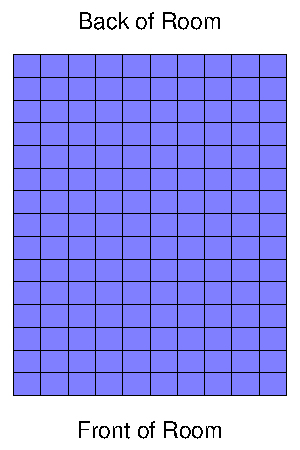
\includegraphics{fullcount}};
\node<1> (srs) at (.75,.5) {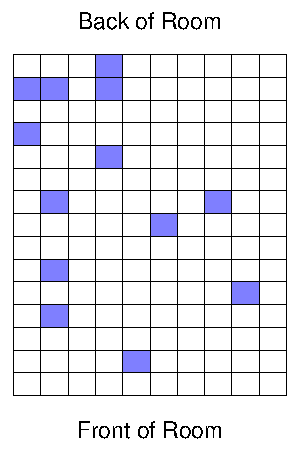
\includegraphics{srs1}};
\node<2> (srs) at (.75,.5) {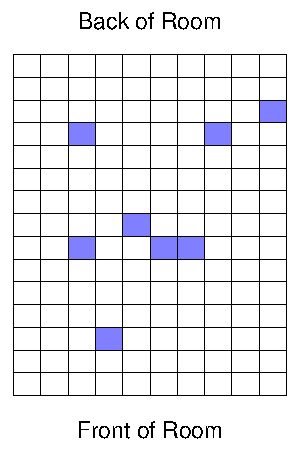
\includegraphics{srs2}};
\node<3> (srs) at (.75,.5) {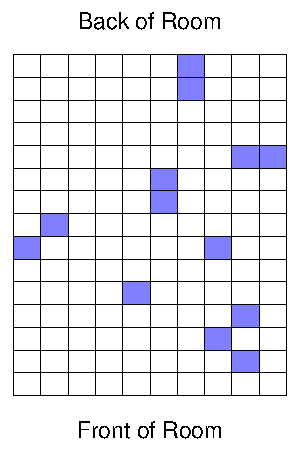
\includegraphics{srs3}};
\node[anchor = south, align = center, font = \bf] at (full.north) {Full Count\\Enumeration};
\node[anchor = south, align = center, font = \bf] at (srs.north) {Probability\\Sample};
\end{tikzpicture}
\end{frame}

\begin{frame}{What are the advantages of each strategy?}
\centering
\scalebox{.8}{
\begin{tikzpicture}[x = \textwidth, y = .8\textheight]
\node (full) at (.25,.5) {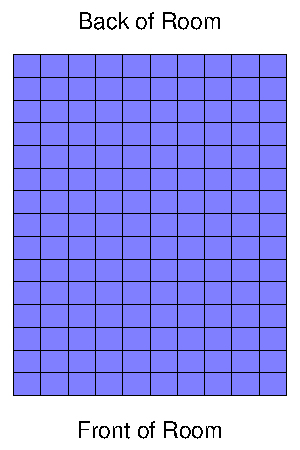
\includegraphics{fullcount}};
\node (srs) at (.75,.5) {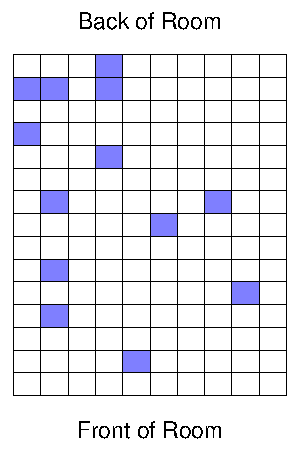
\includegraphics{srs1}};
\node[anchor = south, align = center, font = \bf] at (full.north) {Full Count\\Enumeration};
\node[anchor = south, align = center, font = \bf] at (srs.north) {Probability\\Sample};
\end{tikzpicture}
}
\end{frame}

\begin{frame}{Probability sampling}
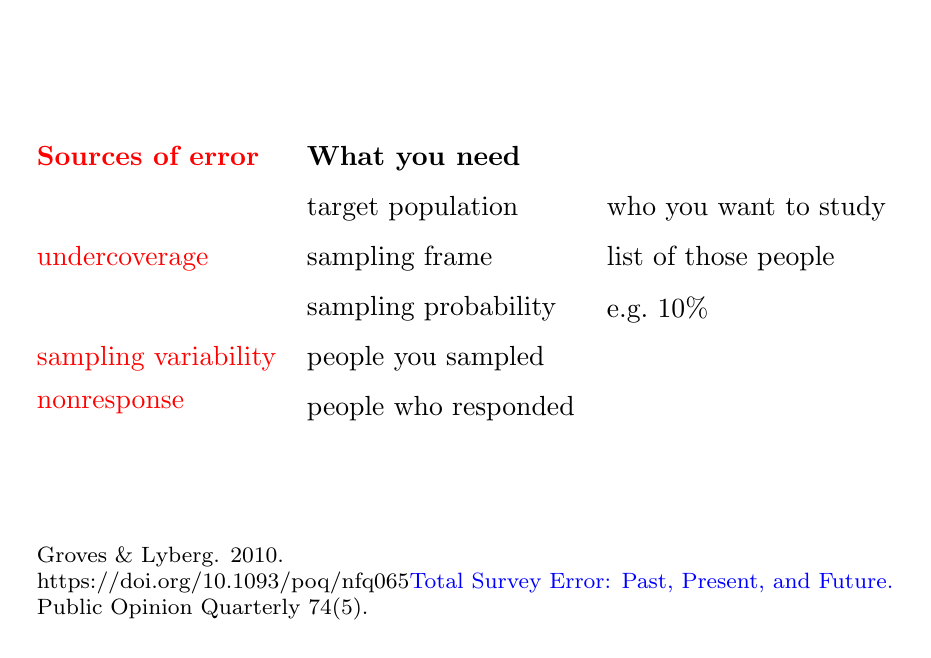
\begin{tikzpicture}[x = 1.5in, y = .25in]
\node at (1,7) {};
\node[anchor = north west, font = \bf] at (1,5) {What you need};
\pause
\node[anchor = north west] at (1,4) {target population};
\node[anchor = north west] at (2,4) {who you want to study};
\pause
\node[anchor = north west] at (1,3) {sampling frame};
\node[anchor = north west] at (2,3) {list of those people};
\pause
\node[anchor = north west] at (1,2) {sampling probability};
\node[anchor = north west] at (2,2) {e.g.~10\%}; 
\pause
\node[anchor = north west] at (1,1) {people you sampled};
\pause
\node[anchor = north west] at (1,0) {people who responded};
\pause
\node[anchor = north west, font = \bf, red] at (.1,5) {Sources of error}; \pause
\node[anchor = north west, red] at (.1,3) {undercoverage}; \pause
\node[anchor = north west, red] at (.1,1) {sampling variability}; \pause
\node[anchor = north west, red] at (.1,0) {nonresponse}; \pause
\node[anchor = north west, font = \footnotesize, align = left] at (.1,-3) {Groves \& Lyberg. 2010.\\\bref{https://doi.org/10.1093/poq/nfq065}{Total Survey Error: Past, Present, and Future.}\\Public Opinion Quarterly 74(5).};
\end{tikzpicture}
\end{frame}

\begin{frame}{Subgroup estimates}
Do the people in the first 3 rows prefer the front? \vskip .2in \pause
Simple random sample
\begin{itemize}
\item everyone run \texttt{runif}
\item everyone respond if $< .1$
\end{itemize} \vskip .2in \pause
Unequal probability sample
\begin{itemize}
\item everyone run \texttt{runif}
\item first 3 rows: respond if $< .5$
\item others: respond if $< .1$
\end{itemize}
\end{frame}

\begin{frame}%{Unequal probability sampling}
\begin{tikzpicture}[x = \textwidth, y = .8\textheight]
\node (design) at (.25,.5) {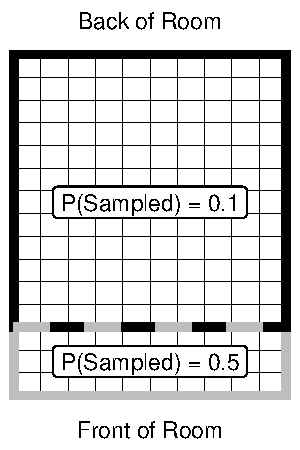
\includegraphics{unequal}};
\node<1> (sample) at (.75,.5) {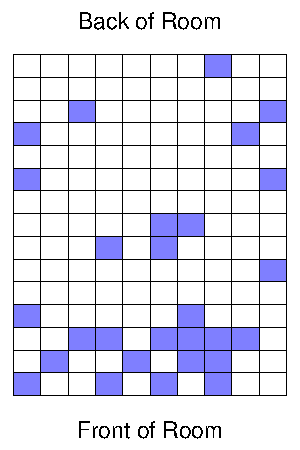
\includegraphics{unequal1}};
\node<2> (sample) at (.75,.5) {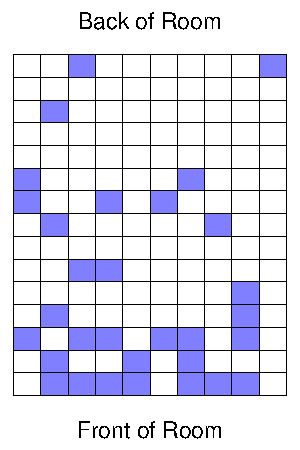
\includegraphics{unequal2}};
\node<3> (sample) at (.75,.5) {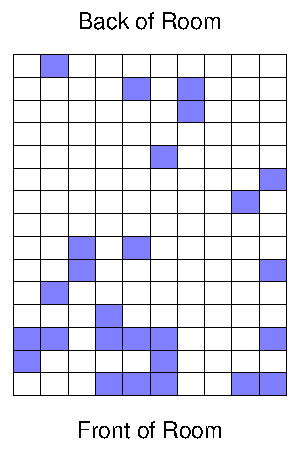
\includegraphics{unequal3}};
\node[anchor = south, align = center, font = \bf] at (design.north) {Sample Design};
\node[anchor = south, align = center, font = \bf] at (sample.north) {Sample};
\end{tikzpicture}
\end{frame}

\begin{frame}
\centering
\begin{tabular}{ll}
full count enumeration & talk to everyone \\ & \onslide<2->{(ideal but costly!)} \\ \\
simple random sample & sampling frame \\ & known, equal probabilities \\ & \onslide<3->{(good for population average)} \\ \\
unequal probability sample & sampling frame \\ & known, unequal probabilities \\ & \onslide<4->{(good for subgroups)}
\end{tabular}
\end{frame}

\begin{frame}

What if we want to estimate the population average\\
from an unequal probability sample?

\begin{center}
\scalebox{.7}{\begin{tikzpicture}[x = \textwidth, y = .8\textheight]
\node (design) at (.25,.5) {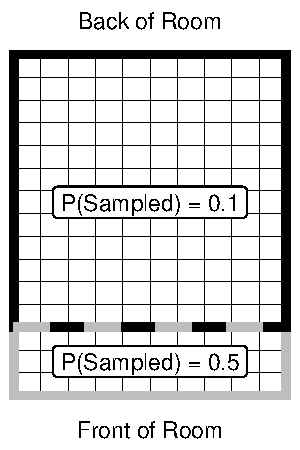
\includegraphics{unequal}};
%\node[anchor = west, font = \Large, align = left] (w) at (-.2,.8) {Sampling\\Weight};
%\draw (w.south west) -- (w.south east);
%\node[anchor = west, font = \Large] at (-.2,.55) {$\frac{1}{.1}$ = 10};
%\node[anchor = west, font = \Large] at (-.2,.2) {$\frac{1}{.5}$ = 2};
\node (sample) at (.75,.5) {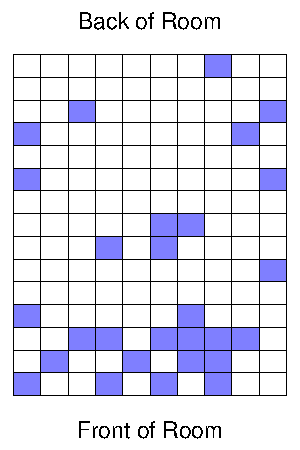
\includegraphics{unequal1}};
\node[anchor = south, align = center, font = \bf] at (design.north) {Sample Design};
\node[anchor = south, align = center, font = \bf] at (sample.north) {Sample};
\end{tikzpicture}}
\end{center}
\end{frame}

\begin{frame}{Sampling weights: Population mean estimator}

Among those sampled if \texttt{runif} $< .1$,\\
on average 1 in 10 people sampled.\\ \pause
Each person represents 10 people.\\ \pause
$w_i = \frac{1}{\P(\text{Sampled})} = \frac{1}{.1} = 10$ \vskip .2in \pause
Among those who sampled if \texttt{runif} $< .5$,\\
on average 1 in 2 people sampled.\\
Each person represents 2 people. \\
$w_i = \frac{1}{\P(\text{Sampled})} = \frac{1}{.5} = 2$  \vskip .2in \pause
$$
\begin{aligned}
& \text{Unweighted estimator} &\qquad& \text{Weighted estimator} \\
& \hat{\E}_\text{Unweighted}(Y) = \frac{\sum_i y_i}{n} &\qquad& \hat{\E}_\text{Weighted}(Y) = \frac{\sum_i w_i y_i}{\sum_i w_i} \\
& \text{(easily misleading!)} & & \text{(correct)}
\end{aligned}
$$

\end{frame}

\begin{frame}
\centering
\begin{tabular}{ll}
full count enumeration & talk to everyone \\ & (ideal but costly!) \\ \\
simple random sample & sampling frame \\ & known, equal probabilities \\ & (good for population average) \\ \\
unequal probability sample & sampling frame \\ & known, unequal probabilities \\ & (good for subgroups) \\ & \bblue{(weight for population average)}
\end{tabular}
\end{frame}

\begin{frame}
\huge
A real question:\\The unemployment rate
\end{frame}

\begin{frame}{A real question: The unemployment rate}

Imagine you are the Bureau of Labor Statistics. \\
How would you design a sample to estimate unemployment?
\begin{enumerate}
\item What would be your sampling frame?
\item How would you define sampling probabilities?
\item What mode of data collection?
\begin{itemize}
\item Mail, phone, web, in person, etc.
\end{itemize}
\item What if people didn't respond?
\end{enumerate}

\end{frame}

\begin{frame}{Current Population Survey: Sample Design}

\begin{center}

\includegraphics[width = .2\textwidth]{bls}
\end{center} \pause

Begin with a \bblue{sampling frame}: all housing units in the U.S.\vskip .1in \pause
\begin{itemize}
\item 1,987 Primary Sampling Units (PSUs)
\begin{itemize}
\item County or contiguous counties within a state
\end{itemize}\vskip .1in \pause
\item Stratified (grouped) within states
\begin{itemize}
\item Stratum: Group of PSUs with similar characteristics
\item One PSU always chosen per stratum
\item \bgray{Why?} Ensure representation across strata
\end{itemize} \vskip .1in \pause
\item Within PSU, sample geographic clusters of housing units
\begin{itemize}
\item \bgray{Why?} Reduce travel costs for field representatives
\end{itemize}
\end{itemize}

\end{frame}

\begin{frame}{Current Population Survey: Sample}

More than 75,000 households are sampled

\end{frame}

\begin{frame}{Current Population Survey: Contacting respondents}

\includegraphics[width = .2\textwidth]{bls}
\includegraphics[width = .3\textwidth]{census-logo}
\begin{enumerate} \vskip .2in \pause
\item Send a letter \pause
\item Call or visit in person \pause
\item Try many times if needed
\end{enumerate} \pause

Learn about the experience for participants \bref{https://www.bls.gov/respondents/cps/home.htm}{here}
\end{frame}

\begin{frame}{Current Population Survey: Mode of Data Collection}
Computer-assisted telephone interview
\begin{center}
\includegraphics<1>[width = .8\textwidth]{cps_questionnaire_1}
\includegraphics<2>[width = .8\textwidth]{cps_questionnaire_2}
\includegraphics<3>[width = .8\textwidth]{cps_questionnaire_3}
\end{center}
\bref{https://www.census.gov/programs-surveys/cps/technical-documentation/questionnaires.html}{census.gov/programs-surveys/cps/technical-documentation/questionnaires.html}
\end{frame}

\begin{frame}{Current Population Survey}{Annual Social and Economic Supplement}

\begin{itemize}
\item Extended survey
\item Conducted each March
\end{itemize} \vskip .1in

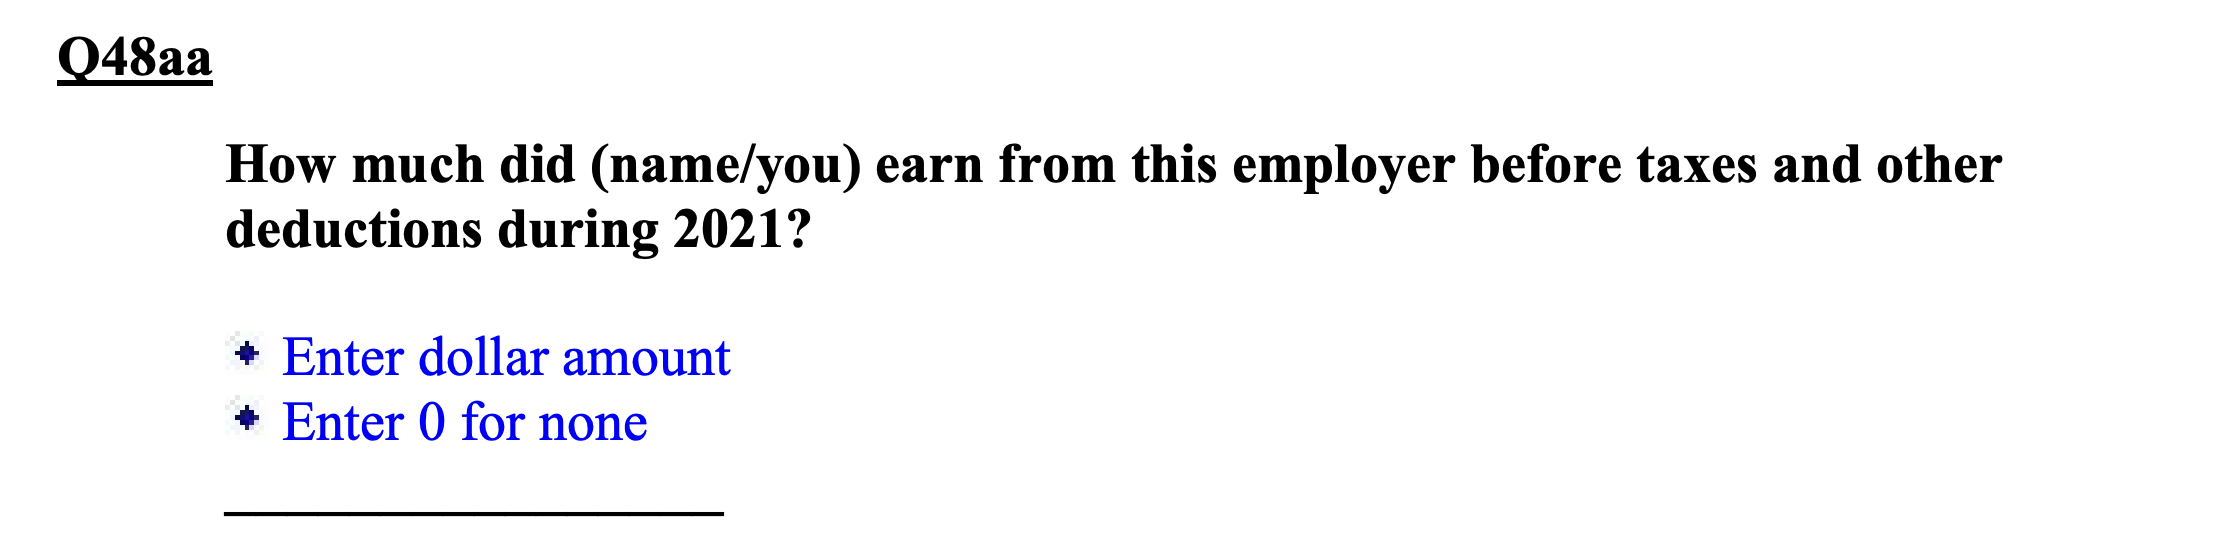
\includegraphics[width = \textwidth]{asec_question} \vskip .3in

\bref{https://www2.census.gov/programs-surveys/cps/techdocs/cpsmar22.pdf}{Questionnaire from 2022}

\end{frame}

\begin{frame}{Rotating panels}
\resizebox{\textwidth}{!}{
    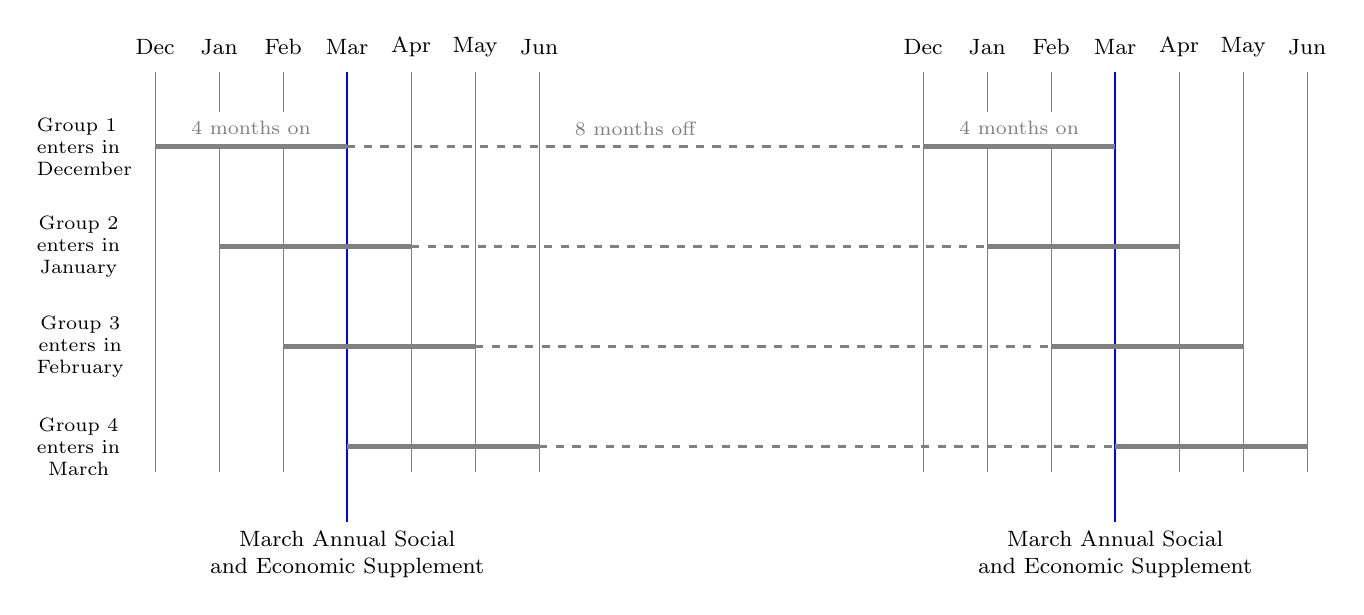
\begin{tikzpicture}[x = .32in, y = .5in]
    \node[font = \footnotesize] at (1,0) {Dec};
    \node[font = \footnotesize] at (2,0) {Jan};
    \node[font = \footnotesize] at (3,0) {Feb};
    \node[font = \footnotesize] at (4,0) {Mar};
    \node[font = \footnotesize] at (5,0) {Apr};
    \node[font = \footnotesize] at (6,0) {May};
    \node[font = \footnotesize] at (7,0) {Jun};
    \node[font = \footnotesize] at (13,0) {Dec};
    \node[font = \footnotesize] at (14,0) {Jan};
    \node[font = \footnotesize] at (15,0) {Feb};
    \node[font = \footnotesize] at (16,0) {Mar};
    \node[font = \footnotesize] at (17,0) {Apr};
    \node[font = \footnotesize] at (18,0) {May};
    \node[font = \footnotesize] at (19,0) {Jun};
    \draw[gray] (1,-.25) -- (1,-4.25);
    \draw[gray] (2,-.25) -- (2,-4.25);
    \draw[gray] (3,-.25) -- (3,-4.25);
    \draw[blue, thick] (4,-.25) -- (4,-4.75);
    \draw[gray] (5,-.25) -- (5,-4.25);
    \draw[gray] (6,-.25) -- (6,-4.25);
    \draw[gray] (7,-.25) -- (7,-4.25);
    \draw[gray] (13,-.25) -- (13,-4.25);
    \draw[gray] (14,-.25) -- (14,-4.25);
    \draw[gray] (15,-.25) -- (15,-4.25);
    \draw[blue, thick] (16,-.25) -- (16,-4.75);
    \draw[gray] (17,-.25) -- (17,-4.25);
    \draw[gray] (18,-.25) -- (18,-4.25);
    \draw[gray] (19,-.25) -- (19,-4.25);
    % First round
    \draw[line width = 2pt, line cap = rounded, gray] (1,-1) to node[midway, above, font = \scriptsize, align = center, fill = white] {4 months on} (4,-1);
    \draw[line width = 2pt, line cap = rounded, gray] (2,-2) -- (5,-2);
    \draw[line width = 2pt, line cap = rounded, gray] (3,-3) -- (6,-3);
    \draw[line width = 2pt, line cap = rounded, gray] (4,-4) -- (7,-4);
    % Period off
    \draw[line width = 1.2pt, line cap = rounded, gray, dashed] (4,-1) to node[midway, above, font = \scriptsize, align = center, fill = white] {8 months off} (13,-1);
    \draw[line width = 1.2pt, line cap = rounded, gray, dashed] (5,-2) -- (14,-2);
    \draw[line width = 1.2pt, line cap = rounded, gray, dashed] (6,-3) -- (15,-3);
    \draw[line width = 1.2pt, line cap = rounded, gray, dashed] (7,-4) -- (16,-4);
    % Second round
    \draw[line width = 2pt, line cap = rounded, gray] (13,-1) to node[midway, above, font = \scriptsize, align = center, fill = white] {4 months on} (16,-1);
    \draw[line width = 2pt, line cap = rounded, gray] (14,-2) -- (17,-2);
    \draw[line width = 2pt, line cap = rounded, gray] (15,-3) -- (18,-3);
    \draw[line width = 2pt, line cap = rounded, gray] (16,-4) -- (19,-4);
    % Label the groups
    \node[align = left, anchor = west, font = \scriptsize] at (-1,-1) {Group 1\\enters in\\December};
    \node[align = left, anchor = west, align = center, font = \scriptsize] at (-1,-2) {Group 2\\enters in\\January};
    \node[align = left, anchor = west, align = center, font = \scriptsize] at (-1,-3) {Group 3\\enters in\\February};
    \node[align = left, anchor = west, align = center, font = \scriptsize] at (-1,-4) {Group 4\\enters in\\March};
    \node[align = center, anchor = north, font = \footnotesize] at (4,-4.75) {March Annual Social\\and Economic Supplement};
    \node[align = center, anchor = north, font = \footnotesize] at (16,-4.75) {March Annual Social\\and Economic Supplement};
    \end{tikzpicture}
}
\end{frame}

\begin{frame}
The Current Population Survey (CPS) is only one of many surveys in the federal statistical system
\end{frame}

\begin{frame}
\centering
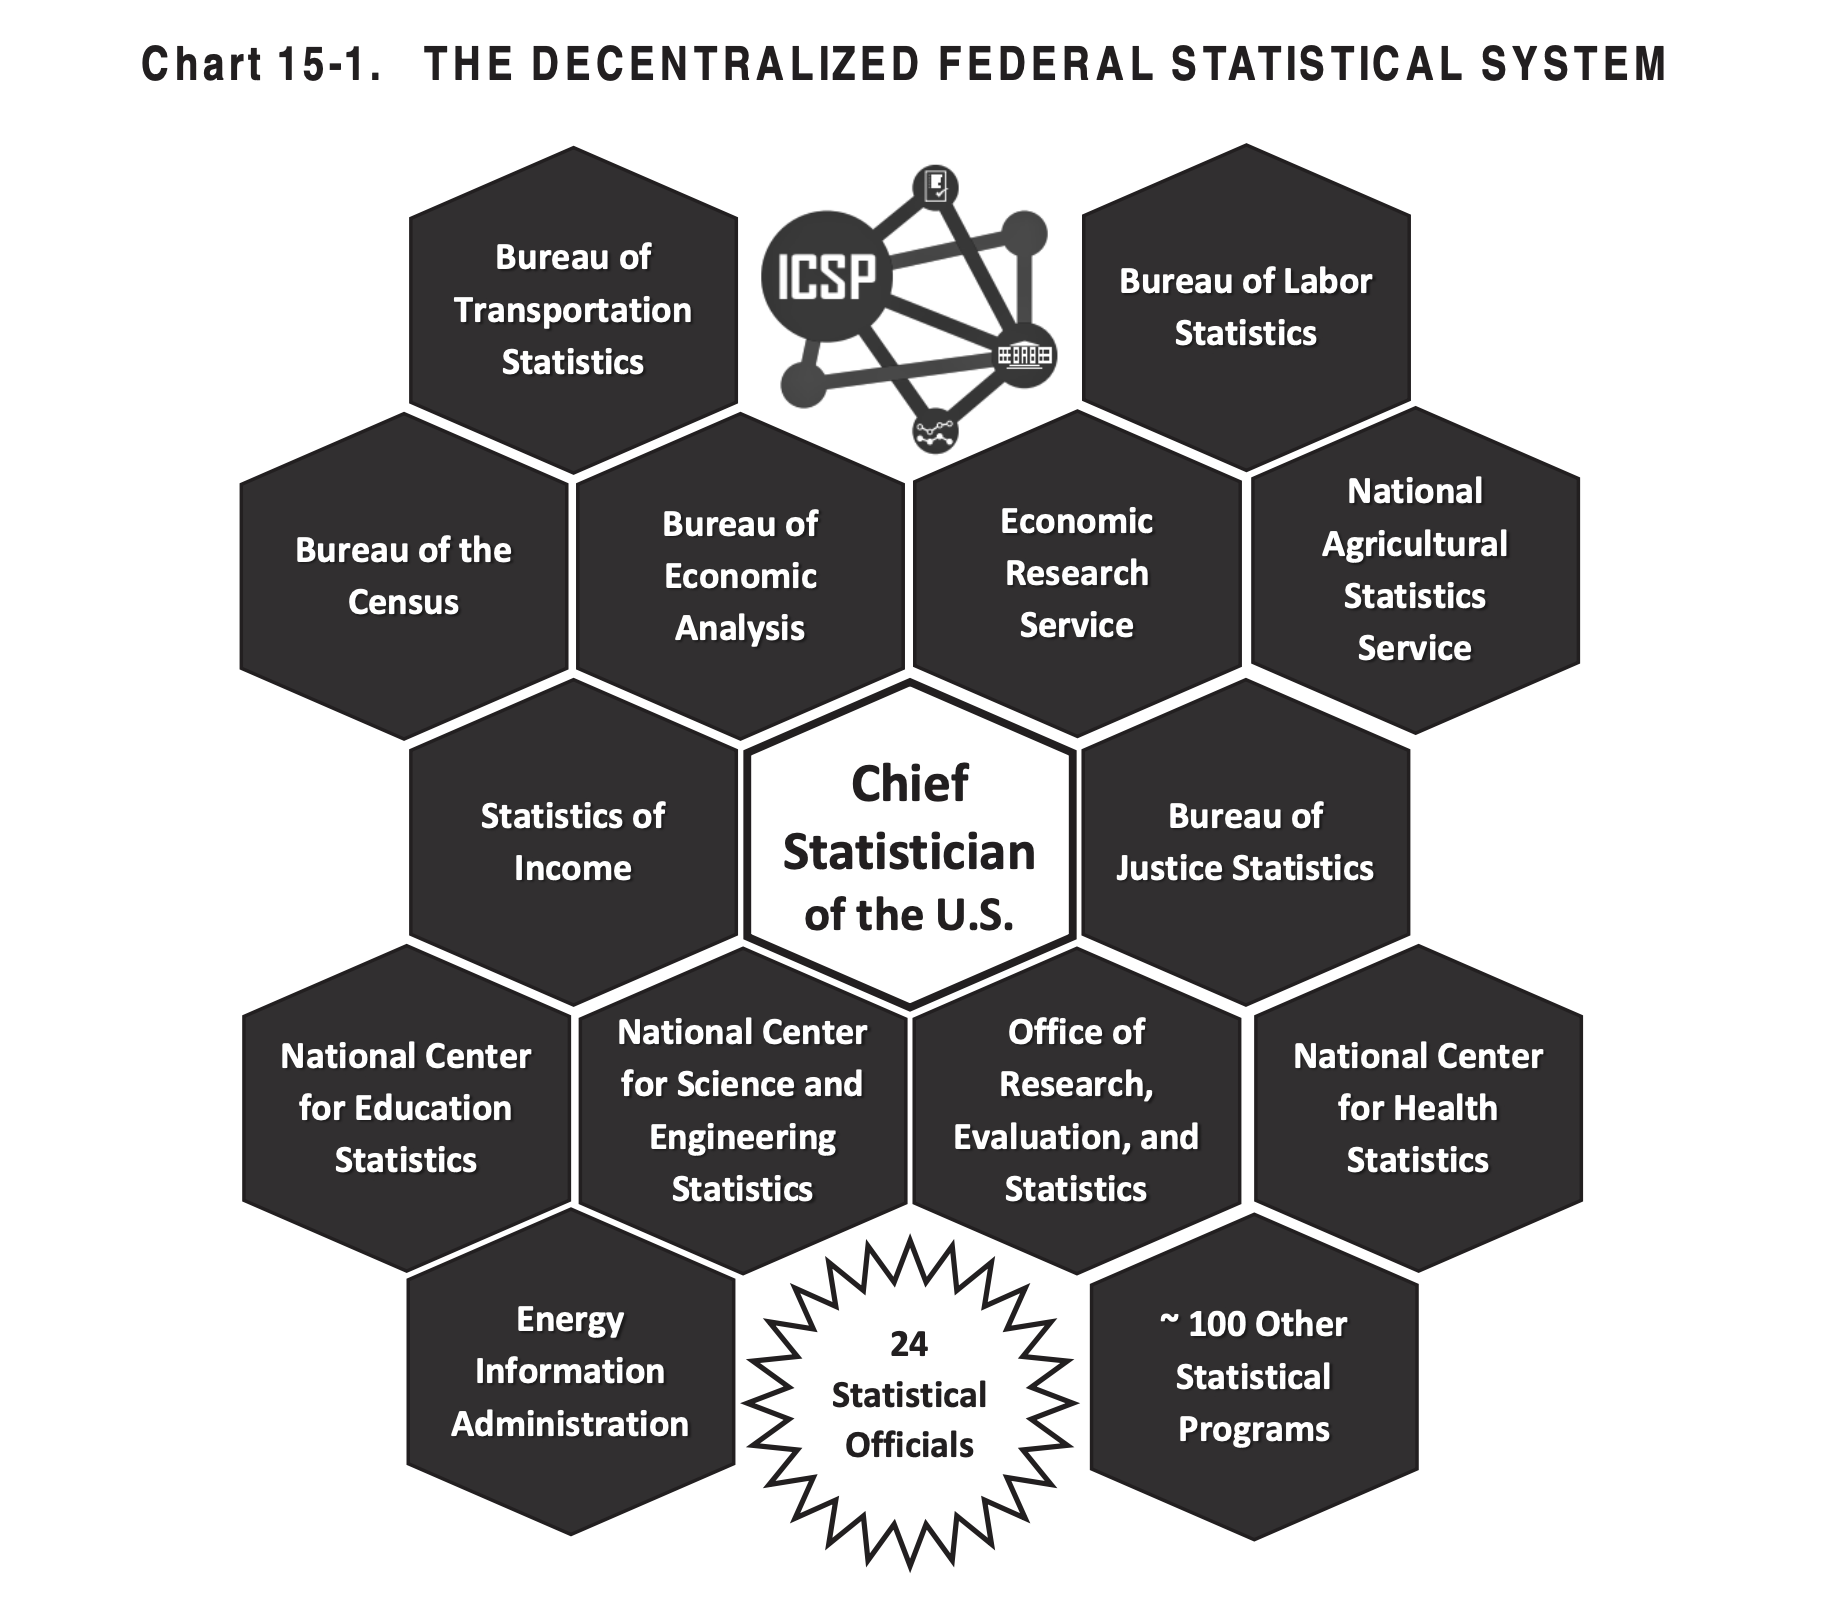
\includegraphics[width = .6\textwidth]{statistical_system} \vskip .3in
\begin{footnotesize}
\bref{https://www.whitehouse.gov/wp-content/uploads/2022/03/ap_15_statistics_fy2023.pdf}{source}
\end{footnotesize}
\end{frame}

\begin{frame}
\begin{center}

\includegraphics[width = .3\textwidth]{ipums_cps}
\end{center}
The Integrated Public Use Microdata Series (IPUMS) distributes these data and more \vskip .1in
\begin{itemize}
\item Easy to access
\item Harmonized documentation
\item Select the variables you want
\item Compare over history
\end{itemize}
\begin{center}

\includegraphics[width = .3\textwidth]{minnesota}
\end{center} \vskip .1in
\begin{tiny}
Sarah Flood, Miriam King, Renae Rodgers, Steven Ruggles, J. Robert Warren and Michael Westberry. Integrated Public Use Microdata Series, Current Population Survey: Version 10.0 [dataset]. Minneapolis, MN: IPUMS, 2022. \bref{https://doi.org/10.18128/D030.V10.0}{https://doi.org/10.18128/D030.V10.0} \par
\end{tiny}
\end{frame}

\begin{frame}
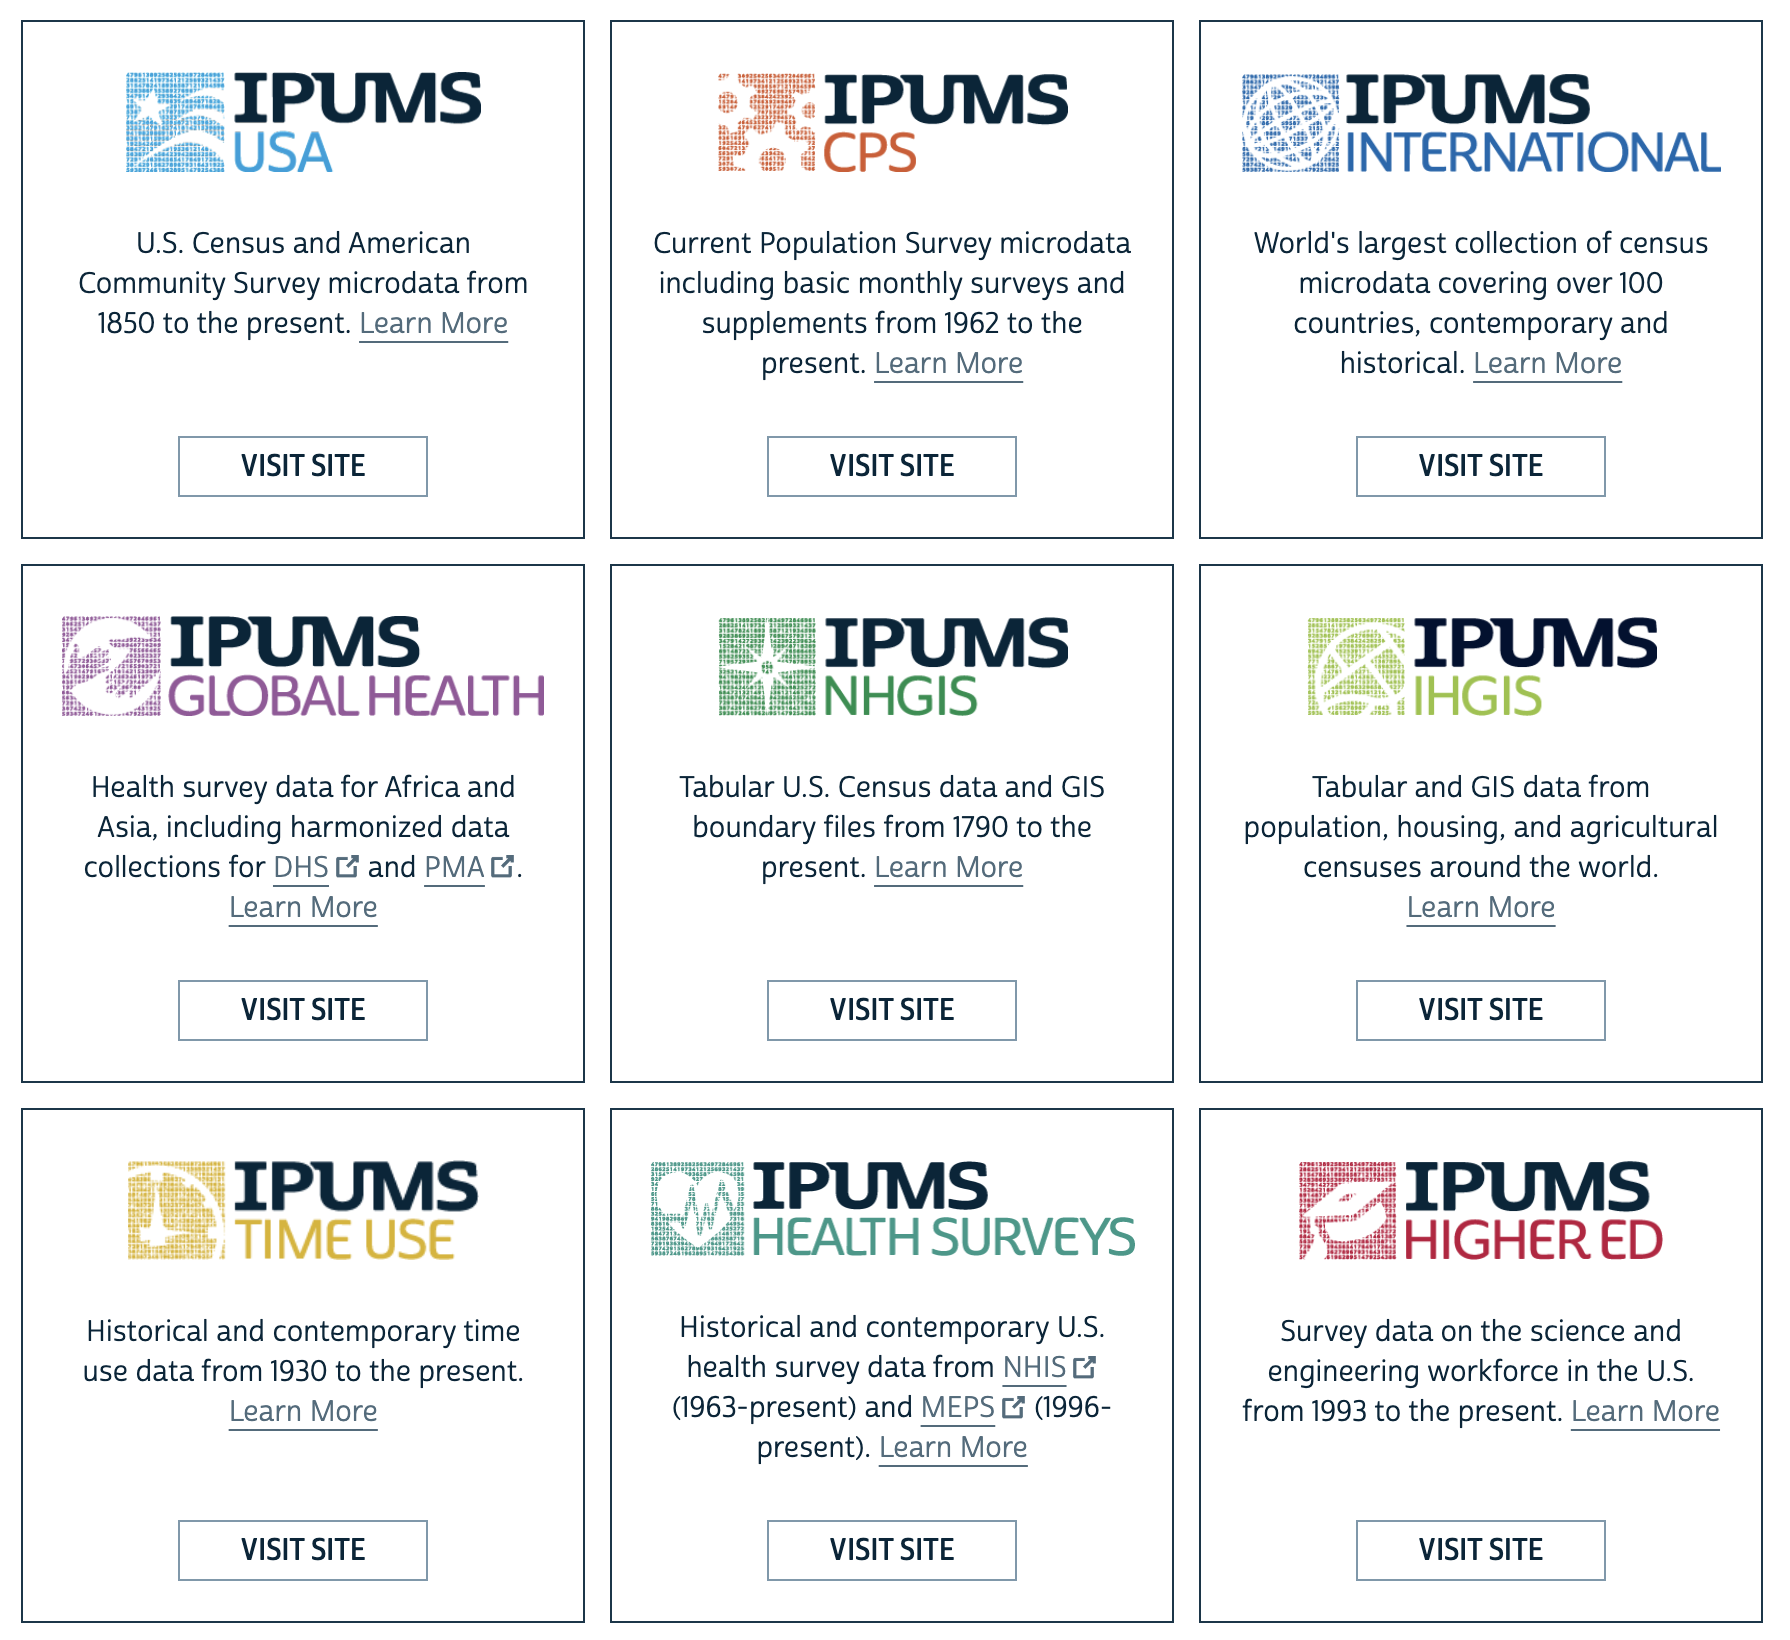
\includegraphics[width = .8\textwidth]{ipums_all}
\end{frame}

\begin{frame}{How to access IPUMS-CPS} \vskip .1in
\begin{tikzpicture}[x = \textwidth, y = .9\textheight]
\node at (0,0) {};
\node at (1,1) {};
\node[anchor = south west] at (0,1) {1) Visit \bref{cps.ipums.org}{https://cps.ipums.org/cps/}. Click \bblue{Register}};
\node[anchor = north west] at (0,1) {
\includegraphics[width = .7\textwidth]{ipums_register_1}};
\draw[->, line width = 2pt, blue] (.6,1.02) -- (.6,.99);
%\draw[->, line width = 2pt, white] (.6,.9) -- (.6,.95);
\node[anchor = south west] at (0,.7) {2) Click \bblue{Apply for access}};
\node[anchor = north west] at (0,.7) {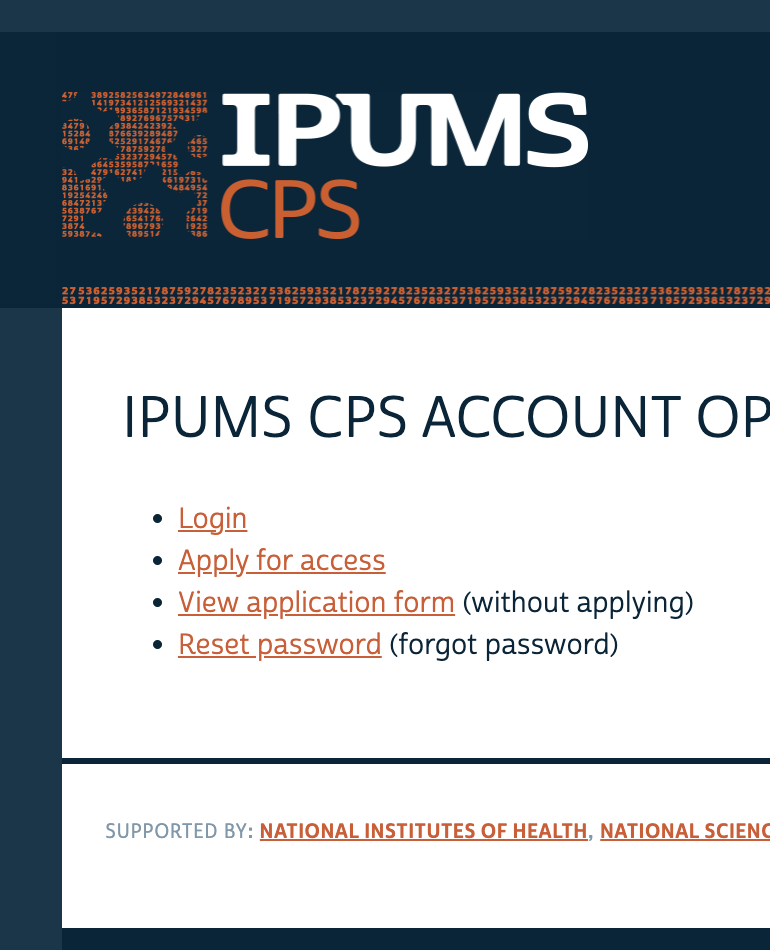
\includegraphics[width = .3\textwidth]{ipums_register_2}};
\draw[->, line width = 2pt, blue] (.23,.45) -- (.18,.42);
\node[anchor = south west] at (.5,.7) {3) Complete the form};
\node[anchor = north west] at (.5,.7) {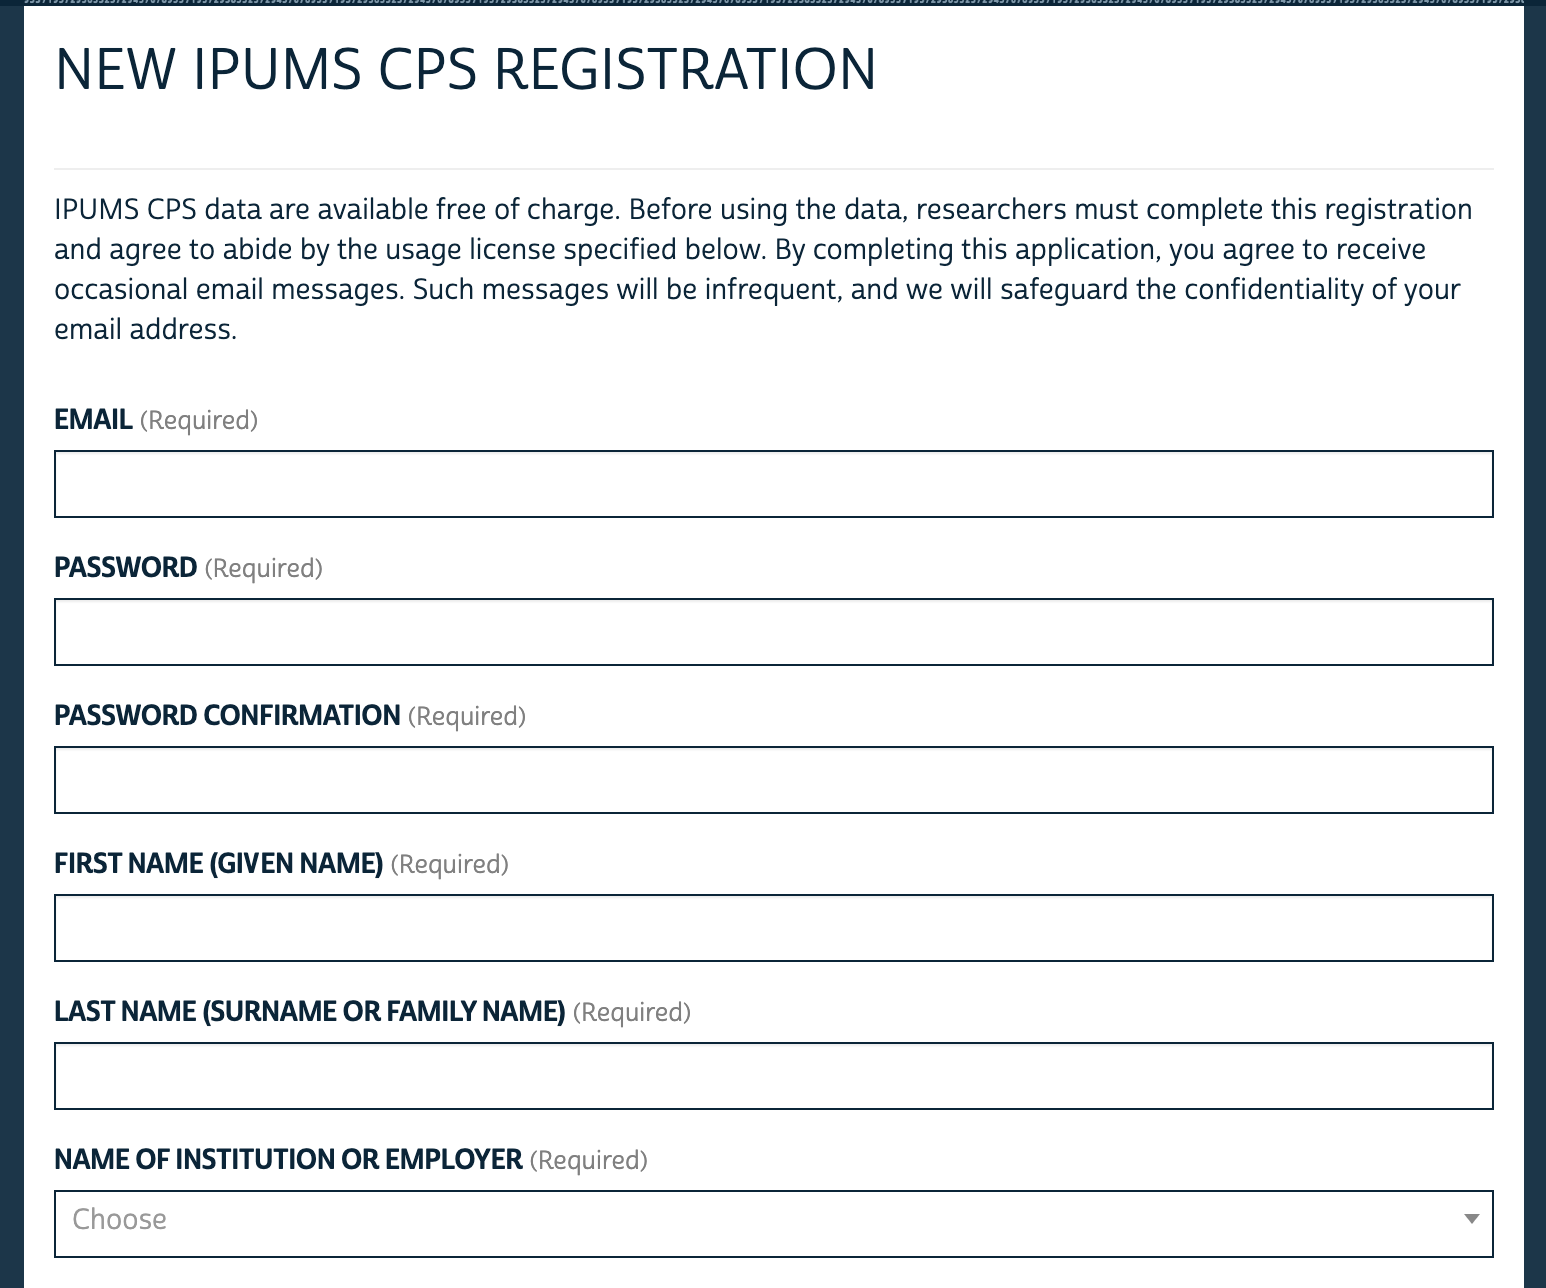
\includegraphics[width = .3\textwidth]{ipums_register_3}};
\node[anchor = north west, text width = .5\textwidth, align = left, font = \footnotesize] at (.5,.35) {General research statement: I am in a class using these data to study socioeconomic inequality in America.};
\end{tikzpicture}
\end{frame}

\begin{frame}{Optional readings}

\begin{itemize}
\item To review central ideas in survey sampling
\begin{itemize}
\item \bref{https://www150.statcan.gc.ca/n1/edu/power-pouvoir/ch13/prob/5214899-eng.htm}{Probability Sampling} from \textit{Statistics: Power from Data!} by Statistics Canada
\end{itemize}
\item For a summary of the total survey error framework
\begin{itemize}
\item \bref{https://www.bitbybitbook.com/en/1st-ed/asking-questions/}{Salganik 2020} 3.1--3.4
\end{itemize}
\item For more information on the Current Population Survey
\begin{itemize}
\item \bref{https://cps.ipums.org/cps/about.shtml}{About CPS}
\item \bref{https://cps.ipums.org/cps/sample_designs.shtml}{CPS Sample Design} which begins about halfway down the page
\end{itemize}
\end{itemize}

\end{frame}

\goalsframe

\end{document}

